\section{The Integers and Rationals}

\subsection{Integers} 

  We then construct the integers as an ordered commutative ring that embeds $\mathbb{N}$ through a canonical ordered monoid homomorphism.  

  \begin{definition}[Integers]
    The \textbf{integers}, denoted with $\mathbb{Z}$ is constructed by defining the equivalence relation on $\mathbb{N} \times \mathbb{N}$ given by 
    \begin{equation}
      (a, b) \sim (c, d) \iff a + d = b + c
    \end{equation}
    which we can think of as $(a, b)$ being the solution to $a = x + b$. We call the quotient set $\mathbb{Z} \coloneqq (\mathbb{N} \times \mathbb{N})/{\sim}$, with the following structure. 
    \begin{enumerate}
      \item \textit{Order} defined by 
        \begin{equation} 
          [(a, b)] \leq_\mathbb{Z} [(c, d)] \iff a + d \leq_\mathbb{N} b + c 
        \end{equation}
      \item \textit{Addition}. 
        \begin{equation}
          [(a, b)] +_{\mathbb{Z}} [(c, d)] \coloneqq [(a + c, b + d)] 
        \end{equation}
      \item \textit{Multiplication}. 
        \begin{equation}
          [(a, b)] \times_{\mathbb{Z}} [(c, d)] \coloneqq [(ac + bd, ad + bc)] 
        \end{equation}

      \item \textit{Additive Identity} is $0$. 
      \item \textit{Multiplicative Identity} is $1$. 
      \item \textit{Additive Inverse} of $z = (a, b) \in \mathbb{Z}$ is denoted $-z = (b, a)$.\footnote{Since $(a, b) + (b, a) = (a + b, a + b) \sim (0, 0)$.}
    \end{enumerate}
    This makes $\mathbb{Z}$ an ordered ring. 
  \end{definition} 
  
  Note that we could have chosen other extensions, but the reason that we choose this is that it preserves the structure of $\mathbb{N}$. Even though set-theoretically, $\mathbb{N}$ and $\mathbb{Z}$ are disjoint, you can embed the naturals in the integers, which aligns with our intuition. 

  \begin{theorem}[Embedding of $\mathbb{N}$ in $\mathbb{Z}$]
    The map $f: \mathbb{N} \rightarrow \mathbb{Z}$ defined $f(n) = [(n, 0)]$ is an ordered monoid homomorphism. That is, it satisfies the following
    \begin{align}
      f(n +_{\mathbb{N}} m) & = f(n)+_{\mathbb{Z}}f(m), \\
      f(n \times_{\mathbb{N}} m) & = f(n)\times_{\mathbb{Z}}f(m) \\
      n\leq m & \iff f(n)\leq_{\mathbb{Z}} f(m)
    \end{align}
  \end{theorem}

  \begin{theorem}[Countability]
    $\mathbb{Z}$ is countably infinite. 
  \end{theorem}

\subsection{Rational Numbers} 

  Just as we have done before, we construct the rationals $\mathbb{Q}$ as an ordered field that embeds $\mathbb{Q}$ through a canonical ordered ring homomorphism. 

  \begin{definition}[Rationals]
    Given the ordered ring of integers $(\mathbb{Z}, +_{\mathbb{Z}}, \times_{\mathbb{Z}}, \leq_{\mathbb{Z}})$ the \textbf{rational numbers} $(\mathbb{Q}, +_{\mathbb{Q}}, \times_{\mathbb{Q}})$ are defined as such. 
    \begin{enumerate}
      \item $\mathbb{Q}$ is the quotient space on $\mathbb{Z} \times \mathbb{Z} \setminus \{0\}$ with the equivalence relation $\sim$ 
      \begin{equation}
        (a, b) \sim (c, d) \iff a \times_{\mathbb{Z}} d = b \times_{\mathbb{Z}} c
      \end{equation} 
      We denote this class as $(a, b)$, where $b > 0$, since if $b < 0$, we know that $(-a, -b)$ are also in this order. 

      \item The additive and multiplicative identities are 
      \begin{equation}
        0_{\mathbb{Q}} \coloneqq (0_{\mathbb{Z}}, a), \;\;\; 1_{\mathbb{Q}} \coloneqq (a, a)
      \end{equation}

      \item Addition on $\mathbb{Q}$ is defined 
      \begin{equation}
        (a, b) +_{\mathbb{Q}} (c, d) \coloneqq \big( (a \times_{\mathbb{Z}} d) +_{\mathbb{Z}} (b \times_{\mathbb{Z}} c), b \times_{\mathbb{Z}} d \big) 
      \end{equation}

      \item The additive inverse is defined 
      \begin{equation}
        -(a, b) \coloneqq (-a, b)
      \end{equation}

      \item Multiplication on $\mathbb{Q}$ is defined 
      \begin{equation}
        (a, b) \times_{\mathbb{Q}} (c, d) \coloneqq \big( a \times_{\mathbb{Z}} c, b \times_{\mathbb{Z}} d \big)
      \end{equation} 

      \item The multiplicative inverse is defined 
      \begin{equation}
        (a, b)^{-1} \coloneqq (b, a)
      \end{equation}

      \item The order $\leq_{\mathbb{Q}}$ defined on the rationals as 
      \begin{equation}
        (a, b) \leq_{\mathbb{Q}} (c, d) \iff ad \leq_{\mathbb{Z}} bc
      \end{equation}
      is a total order. 
    \end{enumerate}
  \end{definition}

  \begin{theorem}[Order on Rationals]
    The order $\leq_{\mathbb{Q}}$ defined on the rationals as 
    \begin{equation}
      (a, b) \leq_{\mathbb{Q}} (c, d) \iff ad \leq_{\mathbb{Z}} bc
    \end{equation}
    is a total order. Remember that we have defined $b, d > 0$. 
  \end{theorem}
  \begin{proof}
    We prove the three properties. 
    \begin{enumerate}
      \item Reflexive. 
      \begin{equation}
        (a, b) \leq_{\mathbb{Q}} (a, b) \iff ab \leq_{\mathbb{Z}} ab
      \end{equation} 

      \item Antisymmetric. 
      \begin{align}
        (a, b) \leq_{\mathbb{Q}} (c, d) & \implies ad \leq_{\mathbb{Z}} bc
        (c, d) \leq_{\mathbb{Q}} (a, b) & \implies bc \leq_{\mathbb{Z}} ad
      \end{align} 
      This implies that both $ad = bc$, which by definition means that they are in the same equivalence class. 

      \item Transitivity. Assume that $(a, b) \leq (c, d)$ and $(c, d) \leq (e, f)$. Then, we notice that $b, d, f > 0$ and therefore by the ordered ring property\footnote{If $a \leq b$ and $0 \leq c$, then $ac \leq bc$.} of $\mathbb{Z}$, we have 
      \begin{align}
        (a, b) \leq_{\mathbb{Q}} (c, d) & \implies ad \leq_{\mathbb{Z}} bc \implies adf \leq_{\mathbb{Z}} bcf \\ 
        (c, d) \leq_{\mathbb{Q}} (e, f) & \implies cf \leq_{\mathbb{Z}} de \implies bcf \leq_{\mathbb{Z}} bde
      \end{align}
      Therefore from transitivity of the ordering on $\mathbb{Z}$ we have $adf \leq bde$. By the ordered ring property\footnote{If $a \leq b$, then $a + c \leq b + c$.}  we have $0 \leq bde - adf = d(be - af)$. But notice that $d > 0$ from our definition of rationals, and therefore it must be the case that $0 \leq be - af \implies af \leq_{\mathbb{Z}} be$, which by definition means $(a, b) \leq_{\mathbb{Q}} (e, f)$. 
    \end{enumerate}
  \end{proof} 

  \begin{theorem}[Rationals are a Field]
    $\mathbb{Q}$ is a field. 
  \end{theorem} 
  \begin{proof}
    We do a few things. 
    \begin{enumerate}
      \item Verify the additive identity. 
      \begin{equation}
        (a, b) + (0, c) = (ac + 0b, bc) = (ac, bc) \sim (a, b)
      \end{equation}
      \item Verify the multiplicative identity. 
      \begin{equation}
        (a, b) \times (c, c) = (ac, bc) \sim (a, b)
      \end{equation}
      \item Additive inverse is actually an inverse. 
      \begin{equation}
        (a, b) + (-a, b) = (ab + (-ba), bb) = (0, bb) \sim (0, 1)
      \end{equation}
      \item Multiplicative inverse is actually an inverse. 
      \begin{equation}
        (a, b) \times (b, a) = (ab, ba) = (ab, ab) \sim (1, 1)
      \end{equation}
      \item Addition is commutative. 
      \begin{equation}
        (a, b) + (c, d) = (ad + bc, bd) = (cb + ad, bd) = (c, d) + (a, b)
      \end{equation}
      \item Addition is associative. 
      \begin{align}
        (a, b) + ((c, d) + (e, f)) & = (a, b) + (cf + de, df) \\
                                   & = (adf + bcf + bde, bdf) \\
                                   & = (ad + bc, bd) + (e, f) \\
                                   & = ((a, b) + (c, d)) + (e, f)
      \end{align}
      \item Multiplication is commutative. 
      \begin{equation}
        (a, b) \times (c, d) = (ac, bd) = (ca, db) = (c, d) \times (a, b)
      \end{equation}
      \item Multiplication is associative. 
      \begin{align}
        (a, b) \times ((c, d) \times (e, f)) & = (a, b) \times (ce, df) \\ 
                                             & = (ace, bdf) \\
                                             & = (ac, bd) \times (e, f) \\
                                             & = ((a, b) \times (c, d)) \times (e, f)
      \end{align}
      \item Multiplication distributes over addition. 
        \begin{align}
          (a, b) \times ((c, d) + (e, f)) & = (a, b) \times (c, d) + (a, b) \times (e, f) \\
                                          & = (ac, bd) + (ae, bf) \\
                                          & = (abcf + abde, b^2 df) \\
                                          & = (acf + ade, bdf)  
                                          & = (a, b) \times (cf + de, df)
        \end{align}
    \end{enumerate}
  \end{proof} 

  \begin{theorem}[Rationals are an Ordered Field]
    $\mathbb{Q}$ is an ordered field. 
  \end{theorem}
  \begin{proof}
    We show that our defined order satisfies the definition. 
    \begin{enumerate}
      \item Assume that $y = (a, b) \leq (c, d) = z$. Let $x = (e, f)$. Then $x + y = (af + be, bf)$, $x + z = (cf + de, df)$. Therefore 
      \begin{align}
        (af + be) df & = adf^2 + bedf \\ 
                     & \leq bcf^2 + bedf \\
                     & = (cf + de) bf
      \end{align} 
      But $(af + be) df = (cf + de) bf$ is equivalent to saying $(af + be, bf) \leq_{\mathbb{Q}} (cf + de, df)$, i.e. $x + y \leq x + z$!  

      \item Let $x = (a, b), y = (c, d)$. Since $0 < x, 0 < y$, by construction this means that $0 < a, 0 < c$ (since $b, d > 0$ in the canonical rational form). By the ordered ring property of the integers, $0 < ac$. So 
      \begin{equation}
        0 < ac \iff 0 \cdot bd < ac \cdot 1 \iff (0, 1) < (ac, bd)  \iff 0_{\mathbb{Q}} < (a, c) \times_{\mathbb{Q}} (b, d) = x y
      \end{equation}
    \end{enumerate}
  \end{proof}

  We have successfully defined the rationals, but now these are almost completely separate elements. We know that all integers are rational numbers, and so to show that the rationals are an extension of $\mathbb{Z}$ we want to identify a \textit{canonical injection} $\iota: \mathbb{Z} \rightarrow \mathbb{Q}$. This can't just be any canonical injection; it must preserve the both the order and algebraic structure between the two sets and must therefore be a \textit{ordered ring homomorphism}. 

  \begin{theorem}[Canonical Injection of $\mathbb{Z}$ to $\mathbb{Q}$ is an Ordered Ring Homomorphism]
    Let us define the canonical injection $\iota: \mathbb{Z} \rightarrow \mathbb{Q}$ to be $\iota(a) = (a, 1)$. This is a ring homomorphism. 
  \end{theorem}
  \begin{proof} 
    We show a few things. 
    \begin{enumerate}
      \item Preservation of addition. 
        \begin{align}
          \iota(a) +_{\mathbb{Q}} \iota(b) & = (a, 1) +_{\mathbb{Q}} (b, 1) \\
                                           & = (1a +_{\mathbb{Z}} 1b, 1^2) \\
                                           & = (a +_{\mathbb{Z}} b, 1) \\
                                           & = \iota(a +_{\mathbb{Z}} b) 
        \end{align}
      \item Preservation of multiplication. 
        \begin{align}
          \iota(a) \times_{\mathbb{Q}} \iota(b) & = (a, 1) \times_{\mathbb{Q}} (b, 1) \\
                                                & = (a \times_{\mathbb{Z}} b, 1^2) \\
                                                & = (a \times_{\mathbb{Z}} b, 1) \\
                                                & = \iota(a \times_{\mathbb{Z}} b, 1)
        \end{align}
      \item Preservation of multiplicative identity. 
        \begin{equation}
          \iota(1_{\mathbb{Z}}) = (1, 1) = 1_{\mathbb{Q}}
        \end{equation}

      \item Preservation of order. 
      \begin{align}
        a \leq_{\mathbb{Z}} b & \iff a \cdot 1 \leq_{\mathbb{Z}} b \cdot 1 \\
                              & \iff (a, 1) \leq_{\mathbb{Q}} (b, 1) \\
                              & \iff \iota(a) \leq_{\mathbb{Q}} \iota(b)
      \end{align}
    \end{enumerate}
  \end{proof} 

  \begin{theorem}[Rational Numbers]
    $\mathbb{Q}$ is countable. 
  \end{theorem}
  \begin{proof}
    Since $\mathbb{N} \approx \mathbb{Z}$, it suffices to prove that $\mathbb{N} \times \mathbb{N}$ is countable. We wish to find the bijection $f: \mathbb{N} \times \mathbb{N} \rightarrow \mathbb{N}$. We claim that 
    \begin{equation}
      f(x, y) = \frac{1}{2} \big\{ (x + y - 1)^2 - (x + y - 1) + 2 \big\} + x - 1
    \end{equation}
    \begin{figure}[H]
      \centering 
      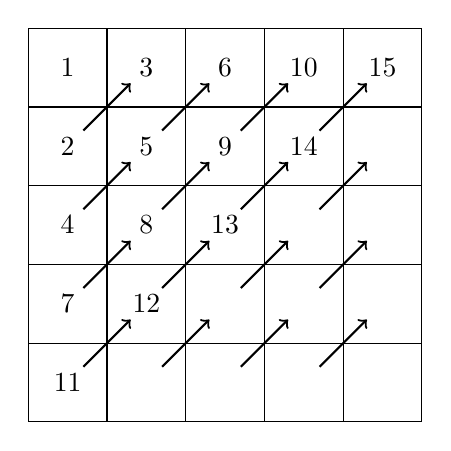
\begin{tikzpicture}[scale=1]
        % Grid
        \draw (0,0) grid (5,5);
        
        % Numbers specified (top-right triangle)
        \node at (0.5,4.5) {1};
        \node at (1.5,4.5) {3};
        \node at (2.5,4.5) {6};
        \node at (3.5,4.5) {10};
        \node at (4.5,4.5) {15};
        
        \node at (0.5,3.5) {2};
        \node at (1.5,3.5) {5};
        \node at (2.5,3.5) {9};
        \node at (3.5,3.5) {14};
        
        \node at (0.5,2.5) {4};
        \node at (1.5,2.5) {8};
        \node at (2.5,2.5) {13};
        
        \node at (0.5,1.5) {7};
        \node at (1.5,1.5) {12};
        
        \node at (0.5,0.5) {11};
        
        % Diagonal arrows
        \foreach \x in {0,...,3} {
            \foreach \y in {0,...,3} {
                \draw[->, thick] (\x+0.7,\y+0.7) -- (\x+1.3,\y+1.3);
            }
        }
      \end{tikzpicture}
      \caption{You can see that given $(x, y)$ it is on the $(x+y+1)$th diagonal, which starts from the $\frac{1}{2} \big((x+y+1)^2 - (x+y+1) + 2)$th number and increments by $x-1$. Therefore, we have the formula above. } 
      \label{fig:rationals_countable}
    \end{figure}
  \end{proof}

  \begin{theorem}[Finite Fields]
    There are no finite ordered fields. 
  \end{theorem} 
  \begin{proof}
    Assume $\mathbb{F}$ is such an ordered field. It must be the case that $0, 1 \in \mathbb{F}$, with $0 < 1$. Therefore, we also have $0 + 1 < 1 + 1 \implies 1 < 1 + 1$. Repeating this we get 
    \begin{equation}
      0 < 1 < 1 + 1 < 1 + 1 + 1 < \ldots
    \end{equation}
    where these elements must be distinct (since only one of $>, <, =$ must be true for a totally ordered set). Since this can be done for a countably infinite number of times, $\mathbb{F}$ cannot be finite. 
  \end{proof}

\subsubsection{Norm, Metric, and Topology on Rationals}

  Note that we can also define a norm on the rationals with just the order and algebraic properties. 

  \begin{theorem}[Norm on $\mathbb{Q}$] 
    The following is indeed a norm on $\mathbb{Q}$. 
    \begin{equation}
      |x| \coloneqq \begin{cases} x & \text{ if } x \geq 0 \\ -x & \text{ if } x < 0 \end{cases}
    \end{equation} 
  \end{theorem} 

  It is well known that the metric induced by any norm is indeed a metric. Therefore we state the metric as a definition. 

  \begin{definition}[Metric on $\mathbb{Q}$]
    The Euclidean metric on $\mathbb{Q}$ is defined 
    \begin{equation}
      d(x, y) \coloneqq |x - y| = \begin{cases} x - y & \text{ if } x \geq y \\ y - x & \text{ if } x < y \end{cases}
    \end{equation}
  \end{definition}

  Thus we get to what we want: the induced topology of open balls. 
  Again, since we know from point-set topology that metric topologies are indeed topologies, we will state this as a definition rather than a theorem.  

  \begin{definition}[Open-Ball Topology on $\mathbb{Q}$]
    The Euclidean topology on $\mathbb{Q}$ is the topology generated by the set $\mathscr{B}$ of all open balls
    \begin{equation}
      B(x, r) \coloneqq \{ y \in \mathbb{Q} \mid |x - y| < r \}
    \end{equation} 
  \end{definition}

  Note that this is the same topology as the order topology. This should however be proved. 

  \begin{theorem}[Metric and Order Topologies on $\mathbb{Q}$]
    The metric and order topologies on $\mathbb{Q}$ are the same topologies. 
  \end{theorem}
  \begin{proof}
    
  \end{proof}

